% !TEX root = TD_fluides_part2.tex


\setcounter{section}{7}

\section{Ecoulements Inertiels II : Ecoulements potentiels}

\setcounter{subsection}{-1}


\subsection{Ecoulement autour d'un cylindre : effet Magnus} 

{\em Correction détaillée sur moodle.}


\vspace{1cm}

On étudie l'écoulement bidimensionnel d'un fluide incompressible de masse volumique uniforme 
$\rho$, défini par le potentiel des vitesses suivant, 
exprimé en coordonnées polaires $(r,\theta)$. :  


  \begin{equation}
   \Phi(r,\theta) =  U_0   \cos \theta \left( r + \frac{a^2}{r}\right)  
   + \frac{\Gamma \theta }{2 \pi}
  \end{equation}
  
Dans cet exercice on néglige la gravité.


\begin{enumerate}
\item Rappelez la définition et les conditions d'existence d'un écoulement potentiel.

\item Exprimez les composantes $u_r, u_\theta$ du champ de vitesse. Vérifiez que l'écoulement est bien à divergence nulle.

\item 
Que deviennent ces expressions sur le cercle de rayon $a$ et à l'infini 
($r \rightarrow \infty$) ? 

Conclure que cet écoulement est solution des équations d'Euler stationnaire
et représente l'écoulement autour d'un cylindre de rayon $a$.

\item Montrez que cet écoulement admet également une fonction de courant définie par
$$
\psi(r,\theta) = U_0   \sin \theta \left( r - \frac{a^2}{r}\right)  
   - \frac{\Gamma}{2 \pi} \ln r/.
 $$
Justifiez que les lignes de courant et les lignes isopotentielles forment des réseaux de courbes orthogonales.

%\item le programme  Matlab \verb|Ecoulement_Potentiel_cylindre.m| 

\item Discutez, suivant la valeur de $\Gamma$, le nombre et la position
des points d'arrêt sur la surface du cylindre (on suppose $\Gamma \leq 0$).

Représentez schématiquement la forme des lignes de courant pour 
différentes valeurs de $\Gamma$.


\item Exprimez le champ de pression $p(r,\theta)$ correspondant à cet écoulement.

Représentez graphiquement la loi de pression pariétale $p(r=a,\theta)$ en fonction de $\theta$,
pour plusieurs valeurs de $\Gamma$.


\item Calculez la force $\vec F$ (par unité de longueur),
exercée par le fluide sur le cylindre. 
Montrez que les composantes $F_x$ et $F_y$ de cette force
 v\'erifient $F_x = 0$ et $F_y = - \rho \Gamma
  U_0$. 
 
 \item Retrouvez ce résultat a partir d'un bilan de quantité de mouvement sur un volume de contrôle judicieusement choisi.
 
   
\item On suppose que le cylindre tourne selon son axe, à la vitesse angulaire
$\Omega$ (c'est à dire que son vecteur rotation est 
$\vec \Omega = \Omega \vec e_z$). 
Donnez, en coordonnées axisymétriques, la  vitesse d'un point situé 
sur la paroi du cylindre. Expliquez pourquoi l'approximation de fluide
parfait ne permet pas de calculer $\Gamma$ en fonction de $\Omega$.


\item L'étude des effets visqueux à l'intérieur de la couche limite {\em (Moore, 1953, Journal of Fluid Mechanics)} permet de montrer que si le cylindre tourne très vite $(\Omega \gg U_0/a)$,  
la circulation est reliée au taux de rotation par $\Gamma = 2 \pi a^2 \Omega$.
Donnez une interprétation physique de cette condition.

\item Montrer que dans ce cas 
$\overrightarrow{F} = 2 \pi \rho a^2 \overrightarrow{U}_0 \wedge \overrightarrow{\Omega}$
(formule de Magnus).

\end{enumerate}


%\subsection{Exercice complémentaire ??? } 

%L'ancien numéro 8, transvasement entre deux réservoirs, est un peu hors sujet...

%Si temps le permet, rajouter l'exercice oscillations dans un tube en U...



\subsection{Oscillations d'un pendule plongé dans un liquide}

Un pendule de masse $M$ attaché à une corde de longueur $L$ est un exemple bien connu d'oscilateur harmonique. Si les interactions avec le fluide sont négligées (ou si le pendule oscille dans le vide) on montre classiquement que la fréquence d'oscillation est donnée par 
$T = 2\pi/\omega_0$ avec $\omega_0 = \sqrt{g/L}$.

Dans le cas où le pendule oscille dans un liquide de masse volumique $\rho$, on observe que la fréquence est modifiée et donnée par la loi suivante :
\begin{equation}
\omega_0^2 = \frac{g (M - \rho V)}{L (M+\rho V C)}
\label{eq:omega0}
\end{equation}

où $V$ est le volume du pendule et $C$ un coefficient appelé "coefficient de masse ajoutée" 
qui dépend de sa forme (et vaut $C=1/2$ pour une sphère et $C=1$ pour un cylindre).



%Dans le cas ou l'oscillateur est un pendule (cylindre de rayon $a$ attaché à une corde de longueur $L$), oscillant dans un liquide, On observe également des différences notables par rapport au cas classique du pendule dans le vide pour lequel 

L'explication de cette modification de la fréquence, ainsi que la prédiction du temps d'amortissement du pendule, on suscité des débats dans la communauté scientifique au milieu du 19ème siècle. C'est Stokes (encore lui...) qui a finalement résolu le problème en 1850. Dans ce problème on va présenter une approche simplifiée de ce travail.


\begin{enumerate}

\subsubsection*{A. Questions préliminaires}


\item
On suppose que l'écoulement peut être modélisé en deux parties : un écoulement extérieur potentiel et une couche limite dominée par les effets visqueux et d'épaisseur $\delta$. 

Rappelez les hypothèses (a verifier a posteriori) permettant de justifier cette approximation.


\item Justifiez que la force exercée par l'écoulement sur la sphère est composée de 3 termes : 
$(i)$ la résultante de pression (motrice) 
$\myvec{F}_p = \iint - \hat{p} \myvec{n} dS$ qui peut être déterminée en fonction de l'écoulement potentiel et non pesant, $(ii)$ la poussée d'Archimède $-\rho V \myvec{g}$, et $(iii)$ l'effet du frottement visqueux $\myvec{F}_v$ dans les couches limites $F_v$.


\subsubsection*{B. Ecoulement potentiel autour d'une sphère en translation}
%On rappelle l'expression des opérateurs gradient et Laplacien en coordonnées sphériques.

La sphère se déplace à vitesse $\myvec{U} =U(t) \myvec{e_x}$ dans une direction $e_x$ supposée fixe.


On note $\myvec u = \gradient \Phi$ le champ de vitesse de l'écoulement {\em dans le repère relatif en mouvement avec la sphère}.

On introduit des coordonnées cartésiennes $x,y,z$ et des coordonnées sphériques 
$r,\theta,\varphi$.



On rappelle les expressions en coordonnées sphériques des opérateurs gradient et Laplacien :

$$
\gradient \Phi = \ddp{\Phi}{r} \myvec{e}_r 
+ \frac{1}{r}\ddp{\Phi}{\theta} \myvec{e}_\theta 
+ \frac{1}{r \sin \theta}\ddp{\Phi}{\varphi} \myvec{e}_\varphi
$$

$$
\Delta \Phi = \frac{1}{r^2} \ddp{}{r} \left( r^2 \ddp{\Phi}{r} \right) 
+ \frac{1}{r^2\sin \theta} \ddp{}{\theta} \left( \sin \theta \ddp{\Phi}{\theta} \right)
+ \frac{1}{r^2\sin^2 \theta} \ddp{^2\Phi}{\varphi^2} 
$$


%\begin{enumerate}
\item Donnez l'équation vérifiée par le potentiel ainsi que les conditions limites vérifiées par ce dernier sur la surface de la sphère ($r=a$) et loin de la sphère ($r \rightarrow \infty$).

\item On cherche une solution à variables séparées sous la forme :
$$
{\color{red} \Phi} (r,\theta) =  f(r) \cos \theta
$$
Donnez l'équation différentielle vérifiée par $f(r)$. 

\item En cherchant des solutions à cette équation sous forme de puissances de $r$, 
montrez que la solution est de la forme $f(r) = A r + B r^{-2}$ où $A$ et $B$ sont des constantes à déterminer.

\item A partir des conditions limites vérifiées en $r=a$ et $r= \infty$ déterminez les constantes $A$ et $B$.

\item En déduire que le champ de vitesse est donné par :

$$
u_r(r,\theta)= -U(t) \left( 1 - \frac{a^3}{r^3} \right) \cos \theta
$$ 
$$
u_\theta(r,\theta)
 = U(t) \left( 1 + \frac{a^3}{2r^3} \right) \sin \theta
 $$

Représentez schématiquement la structure de l'écoulement.

\subsubsection*{C. Champ de pression et force exercée sur la sphère due à l'écoulement potentiel}

Dans cette partie on ne tient pas compte de la gravité et du frottement visqueux, on s'intéresse uniquement à la force exercée par la sphère associée à l'écoulement potentiel.

%\item Justifiez que la force exercée par la sphère se décompose en 3 termes :
%$(i)$ une force hydrodynamique que l'on peut calculer a partir de 

\item A partir des équations d'Euler dans le repère relatif en mouvement avec la sphère ({\em non galliléen)}, démontrer une forme généralisée du second théorème de Bernouilli.

\item En déduire l'expression de la pression $p(a,\theta)$ exercée sur la surface du cylindre. 

\item Montrez que la force exercée sur l'objet par l'écoulement vaut :
$$
\myvec{F}_p = - \rho V C  \frac{ dU}{dt} \myvec{e}_x  , \quad \mbox{ avec } V = \frac{4 \pi a^3}{3} \mbox{ et } 
C = \frac{1}{2}
$$
%$$
%F_y = 0
%$$
%Quelle est l'interprétation physique des deux termes apparaissant dans $F_x$ ?

\item Que vaut la force si la sphère se déplace à vitesse uniforme ? Commentez ce résultat.

\item Que vaut la force si la sphère se déplace de manière uniformément accélérée ? Interprétez physiquement le résultat et donnez une interprétation géométrique au coefficient $C$.


\subsubsection*{D. Application : oscillations d'un pendule}

On considère maintenant le cas d'un pendule constitué d'une sphère de rayon $a$ et masse $m$ attaché à une ficelle de longueur $L$. 

On note $\phi(t)$ l'angle d'inclinaison du pendule, et on introduit un repère 
$(\myvec{e}_x, \myvec{e}_y, \myvec{e}_z)$ tel que la vitesse instantanée soit alignée avec l'axe $x$, c.a.d. : $\myvec{U} = U(t) \myvec{e}_x = L d \phi / dt$.

On admettra qu'on peut négliger les termes d'accélération centrifuge et de Coriolis, et que l'écoulement autour de la sphère et la force associé sont les mêmes que ce qu'on a calculé dans les questions précédentes.




\item En appliquant le principe fondamental de la dynamique à la sphère, projeté selon l'axe 
$\myvec{e_x}$, montrez que le mouvement est gouverné par l'équation différentielle suivante :

$$
(m+\rho VC) L
\frac{d^2 \phi}{d t^2} =  \myvec{F}_v \cdot \myvec{e_x} { \color{red} - }  (m-\rho V) g \phi
$$



\item Si les forces visqueuses sont négligeables, en déduire que le pendule oscille avec la période $T = 2\pi / \omega_0$ où $\omega_0$ est donné plus haut par l'équation (\ref{eq:omega0}).

\item 
Application numérique : calculez la période pour un pendule de dimensions $L=10cm$, $a=1cm$, dans les cas suivants :

$(i)$ Pendule en acier ($\rho_p = 7850$) dans l'eau ($\rho = 1000$)

$(ii)$ Pendule en PVC ($\rho_p = 1400$) dans l'eau ($\rho = 1000$)

$(ii)$ Pendule en verre ($\rho_p = 2500$) dans l'air ($\rho = 1.225$)

\subsubsection*{E. Estimation des effets visqueux}

\item Estimez l'épaisseur de la couche limite $\delta$ dans les 3 cas précédents. L'hypothèse de couche limite est-elle effectivement justifiée a posteriori ?

\item Dans le cas d'une sphère oscillant à la pulsation $\omega_0$, le calcul des forces de frottement dans les couches limites (du à Stokes) conduit à :

$$
\myvec{F}_v = - \frac{9}{4} \frac{V}{a}  \mu \frac{U(t)}{\sqrt{\frac{\nu}{\omega_0}}} \myvec{e}_x
$$   

Justifiez la forme de cette expression (on ne demande pas de démontrer le facteur 9/4 !).

\item
En supposant que l'effet des frottements visqueux est une petite correction par rapport au calcul précédent, montrez que l'on aboutit à une équation d'oscillateur harmonique amorti de la forme :

$$
\frac{d^2 \phi}{d t^2} + \frac{1}{\tau} \frac{d \phi}{d t} + \omega_0^2 \phi =0
$$

\item Donnez la valeur du temps d'amortissement $\tau$ du pendule pour les cas $(i)$, $(ii)$ et $(iii)$ définis plus haut.

\end{enumerate}


\comment{

%--------------------------------------------------------------------------------------------------
\subsection{Ascension d'une bulle parachute (d'après Davies \& Taylor, 1950) $^*$}
%--------------------------------------------------------------------------------------------------

\begin{figure}[hbt]
  \begin{center}
    \setlength{\unitlength}{1mm}
    \begin{picture}(100, 110)(0, 5)
      \put(0, 61){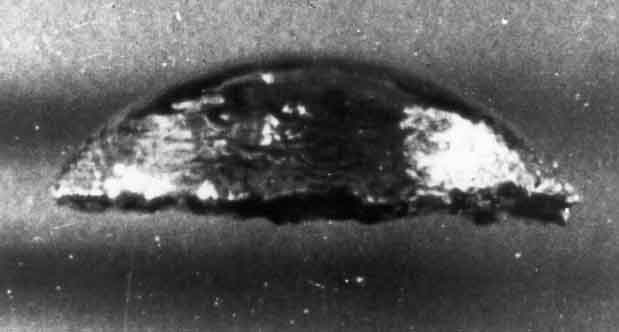
\includegraphics[width=7cm]{bubble_cap1}}
      \put(0, 0){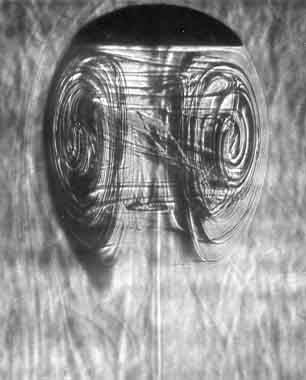
\includegraphics[height=4cm]{bubble_cap2}}
      \put(50, 0){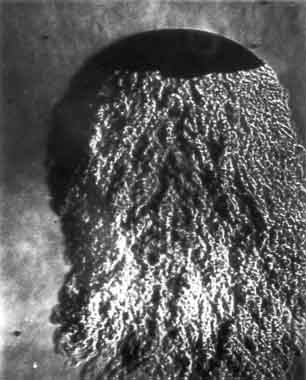
\includegraphics[height=4cm]{bubble_cap3}}
      \put(2, 109){\bf (a)}
      \put(2, 3){\bf (b)}
      \put(52, 3){\bf (c)}
    \end{picture}
  \end{center}
  \mycaption{(a) Photographie d'une bulle parachute en ascension
    (Davenport \textit{et al.}, 1967).
    Bulle avec sillage laminaire \`a $Re=180$ (b) et turbulent \`a $Re = 17000$ (c).
    D'après Wegener \& Parlange (1973).}
  \label{fig:cap_bubbles}
\end{figure}


\begin{figure}
  \begin{center}
%   \setlength{\unitlength}{1mm}
%    \begin{picture}(60, 65)(0, 5)
%      \put(0, 0){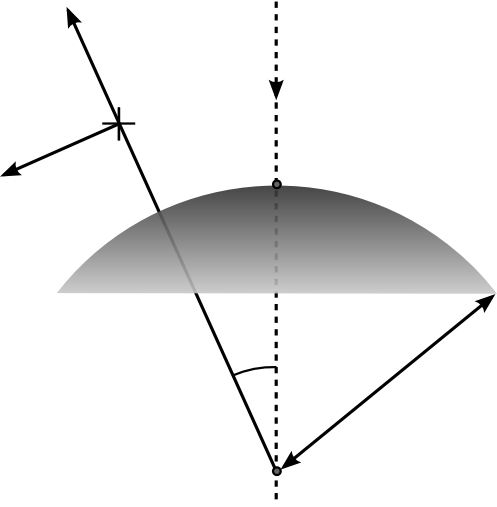
\includegraphics[width=6cm]{geometrie_bulle.png}}
%      \put(29, 3){$O$}
%      \put(2, 44){$\vec{e}_\theta$}
%      \put(12, 58){$\vec{e}_r$}
%      \put(30, 18){$\theta$}
%      \put(24, 21){\colorbox{white}{$r$}}
%      \put(29.5, 40){$S$}
%      \put(44.5, 14){\colorbox{white}{$R$}}
%      \put(16, 48){$M$}
%    \end{picture}
\vspace{-9cm}
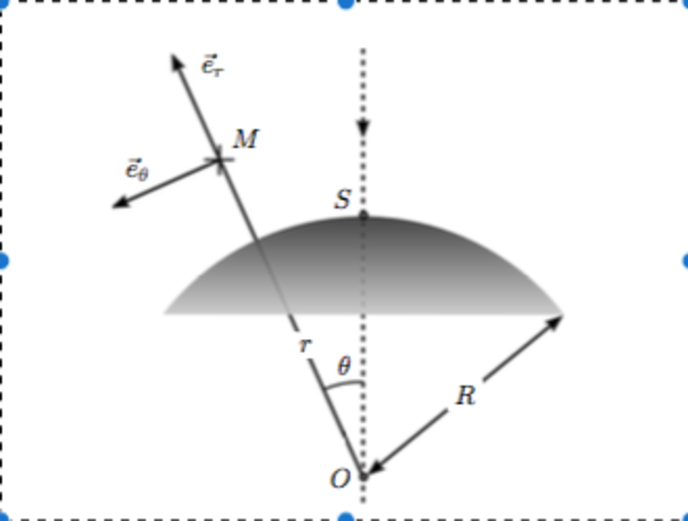
\includegraphics[width=15cm]{BulleTaylorShema.pdf}
\vspace{-8cm}
  \end{center}
  \mycaption{Param\`etres g\'eom\'etriques de l'\'ecoulement autour d'une bulle.}
  \label{fig:geometrie_bulle}
\end{figure}


L'exp\'erience montre que les bulles de gaz de quelques centim\`etres de diam\`etre qui remontent 
dans un liquide ont une forme de parachute (fig.~\ref{fig:cap_bubbles})~:
la partie avant de la bulle est sph\'erique et sa partie arri\`ere
est \`a peu pr\`es plate (calotte sph\'erique).
G. I. Taylor a \'etudi\'e exp\'erimentalement la relation entre la vitesse
d'ascension des bulles et le rayon de courbure de la partie avant.
Dans ses exp\'eriences, des bulles d'air s'\'el\`event dans du nitrobenz\`ene
(de viscosit\'e cin\'ematique $\nu = 0.015$ cm$^2$/s et de masse volumique
$\rho = 1.2$ g/cm$^3$).
Les rayons de courbures observ\'es sont compris entre $2.4$ et $4.8$ cm,
les vitesses d'ascension correspondantes entre $29$ et $48$ cm/s
et les dimensions transverses $2R\sin\theta_m$ entre $2.8$ et $6.2$ cm.

\begin{enumerate}

\item 
Dans les exp\'eriences d\'ecrites ci-dessus, quel est l'ordre de grandeur du nombre de Reynolds 
pour l'\'ecoulement de liquide ?
Conclusions.

\item Evaluez le nombre de Bond. En déduire que la pression le long de la surface de la bulle peut être considérée comme constante.


\item A partir du théorème de Bernouilli, donner une relation entre l'altitude 
$z= R \cos \theta$  et la vitesse $|\vec{u}(R,\theta)|$ sur la surface de la bulle.


%Evaluer la vitesse tangentielle du liquide au voisinage du point d'arr\^et $S$. 
%On pourra supposer que la pression \`a l'int\'erieur de la bulle est constante.

\item 
Taylor fait la remarque que l'\'ecoulement du liquide autour du sommet
de la calotte sph\'erique est peu diff\'erent de l'\'ecoulement potentiel
autour d'une sph\`ere donn\'e par
$$
u_r(r, \theta) = -U\left ( 1 - \frac{R^3}{r^3} \right ) \cos\theta
\quad \mbox{et} \quad
u_\theta(r, \theta) = U\left ( 1 + \frac{R^3}{2r^3} \right ) \sin \theta
$$
dans le r\'ef\'erentiel o\`u la bulle est immobile et o\`u le liquide
se d\'eplace \`a la vitesse $U$ loin de la bulle. 

%
%En comparant ces expressions avec les r\'esultats obtenus pr\'ec\'edemment, 
%d\'eterminer la vitesse d'ascension de la bulle. 


En déduire que la vitesse de la bulle est donnée par :
$$
U = \frac{2}{3} \sqrt{gR}
$$

\item
Confronter cette pr\'ediction th\'eorique aux valeurs obtenues exp\'erimentalement.

\end{enumerate}

% R\'ef\'erence : \cite[\S 6.11]{Bat67}


%\noindent \textbf{R\'ef\'erences bibliographiques}

% Davenport W.G., Bradshaw A.V. \& Richardson F.D. (1967) 
% Behavior of spherical-cap bubbles in liquid metals.
% \textit{J. Iron Steel Inst.} \textbf{205}, 1034--1042.

% Davies R.M. \& Taylor G.I. (1950)
% The mechanics of large bubbles rising through extended liquids and through liquids in tubes.
% \textit{Proc. Roy. Soc. A} \textbf{200}, 375--390.

% Wegener P.P. \& Parlange J.-Y. (1973) 
% Spherical-cap bubbles.
% \textit{Annu. Rev. Fluid Mech.} \textbf{5}, 79--100.



}







